%-------------------------
% Resume in Latex
% Template: Sourabh Bajaj
% Author: Lukas Grams
% License : MIT
%------------------------

\documentclass[letterpaper,11pt]{article}

\usepackage{latexsym}
\usepackage[empty]{fullpage}
\usepackage{titlesec}
\usepackage{marvosym}
\usepackage[usenames,dvipsnames]{color}
\usepackage{verbatim}
\usepackage{enumitem}
\usepackage{xcolor}
\usepackage[colorlinks=true, urlcolor=blue, pdfborderstyle={/S/U/W 1},pdfborder=0 0 1, urlbordercolor=blue ]{hyperref}
%\usepackage[hidelinks]{hyperref}
%\usepackage{hyperref}
\usepackage{fancyhdr}
\usepackage{nccfoots}
\usepackage{graphicx}
\graphicspath{{C:/Users/GSYS/Downloads/} }
\usepackage{float}


\pagestyle{fancy}
\fancyhf{} % clear all header and footer fields
\fancyfoot{}
\renewcommand{\headrulewidth}{0pt}
\renewcommand{\footrulewidth}{0pt}

% Adjust margins
\addtolength{\oddsidemargin}{-0.5in}
\addtolength{\evensidemargin}{-0.5in}
\addtolength{\textwidth}{1in}
\addtolength{\topmargin}{-.5in}
\addtolength{\textheight}{1.0in}

\urlstyle{same}

\raggedbottom
\raggedright
\setlength{\tabcolsep}{0in}

% Sections formatting
\titleformat{\section}{
  \vspace{-4pt}\scshape\raggedright\large
}{}{0em}{}[\color{black}\titlerule \vspace{-5pt}]

%-------------------------
% Custom commands
\newcommand{\resumeItem}[2]{
  \item\small{
    \textbf{#1}{: #2 \vspace{-2pt}}
  }
}

\newcommand{\resumeItemWithoutHeadline}[1]{
	\item\small{
		{#1 \vspace{-2pt}}
	}
}

\newcommand{\resumeSubheading}[4]{
  \vspace{-1pt}\item
    \begin{tabular*}{0.97\textwidth}[t]{l@{\extracolsep{\fill}}r}
      \textbf{#1} & #2 \\
      \textit{\small#3} & \textit{\small #4} \\
    \end{tabular*}\vspace{-5pt}
}

\newcommand{\resumeSubItem}[2]{\resumeItem{#1}{#2}\vspace{-4pt}}

\renewcommand{\labelitemii}{$\circ$}

\newcommand{\resumeSubHeadingListStart}{\begin{itemize}[leftmargin=*]}
\newcommand{\resumeSubHeadingListEnd}{\end{itemize}}
\newcommand{\resumeItemListStart}{\begin{itemize}}
\newcommand{\resumeItemListEnd}{\end{itemize}\vspace{-5pt}}

%-------------------------------------------
%%%%%%  CV STARTS HERE  %%%%%%%%%%%%%%%%%%%%%%%%%%%%

\begin{document}

%----------HEADING-----------------
\begin{tabular*}{\textwidth}{l@{\extracolsep{\fill}}r}
  	\textbf{\Large Lukas Grams}\\
	{Geburtsdatum: 20.09.1994}\\
  	{Wohnort: Rosenheim}\\
  	{Tel : +49 151 6519 6156}\\  
	\big[
	\href{https://www.xing.com/profile/Lukas_Grams/cv}{Xing},
	\href{https://github.com/gramsimamsi/}{github},
	\href{https://www.linkedin.com/in/lukas-grams/?locale=de}{linkedin (de)},
	\href{https://www.linkedin.com/in/lukas-grams/?locale=en_US}{linkedin (eng)} 
	\vspace*{-2.6cm}	
	\big] \\
	Email : \href{mailto:lukas.grams.info@gmail.com}{lukas.grams.info@gmail.com} &
	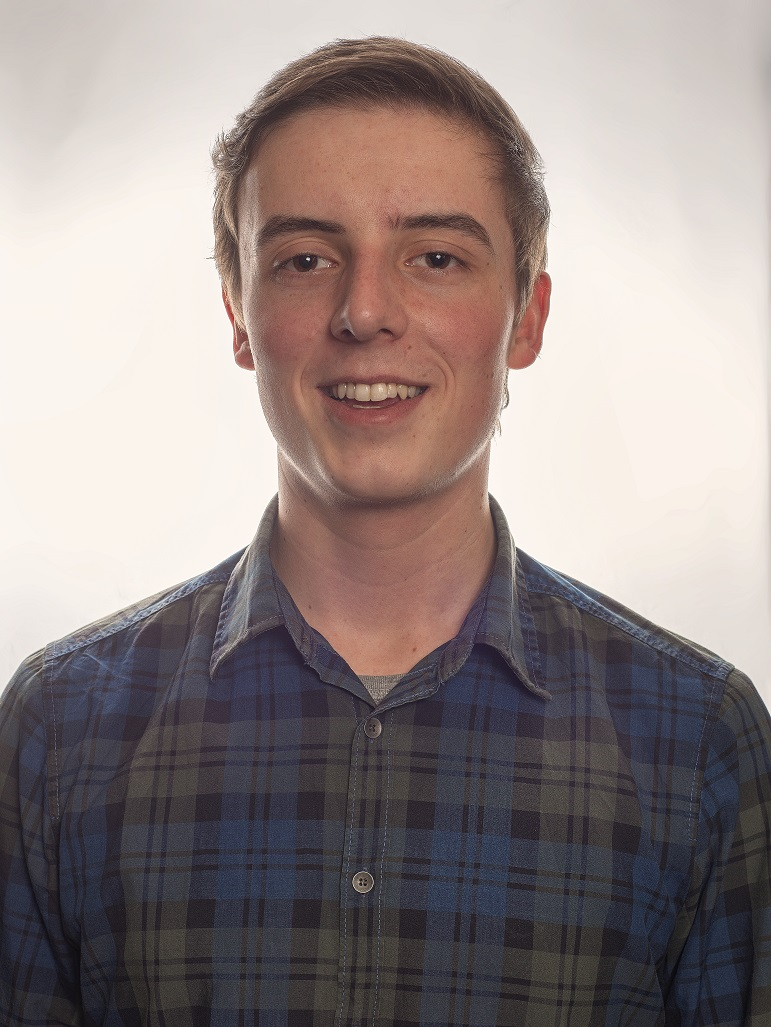
\includegraphics[scale=0.35]{Passbild.jpg}\\	
\end{tabular*}

%-----------EDUCATION----------------
\section{Ausbildung}
  \resumeSubHeadingListStart
    \resumeSubheading
   	  {B. Sc. Informatik im aktuell 7. Semester}{2015 -- heute}    
      {Hochschule Rosenheim,  vorl. Bachelor-Schnitt: 1,6}{Rosenheim}
  	\resumeSubheading
  	  {Schulabschluss Fachhochschulreife}{2014 -- 2015}
      {Berufsoberschule Wasserburg am Inn,  Notenschnitt: 2,0}{Wasserburg}
    \resumeSubheading
      {Abgeschlossene Berufsausbildung IT-Systemelektroniker (IHK)}{2011 -- 2014}
      {Berufsschule München,  Notenschnitt: 1,0}{München}
  \resumeSubHeadingListEnd

%-----------EXPERIENCE-----------------
\section{Berufserfahrung}
  \resumeSubHeadingListStart

	\resumeSubheading
	{Technical Specialist im Vulnerability Management}{2018 - heute}
  	{Fujitsu Technology Solutions}{München}
  	\resumeItemListStart
		\resumeItemWithoutHeadline
       	{Entwickeln von Tools, Systemen und Prozessen zur Automatisierung \linebreak
   		von Vulnerability Management Analysen und Alertings}
        \resumeItemWithoutHeadline
		{Verwendete Technologien: Docker, Git/GitLab, Ruby, Shell-Scripts, Ubuntu, RHEL, \linebreak
		Elasticsearch, Logstash, Kibana, Kolide Fleet, Osquery}
	\resumeItemListEnd

	\resumeSubheading
	{Tutor / Übungsleiter für  Algorithmen \& Datenstrukturen, Programmieren 2}{2017 - 2018}
	{Hochschule Rosenheim, Fakultät Informatik}{Rosenheim}
	\resumeItemListStart
		\resumeItemWithoutHeadline
		{Programmieren 2: \linebreak
			Anleiten und Beraten der Studenten in fortgeschrittenen Konzepten der objektorientierten Programmierung \linebreak
			(Java, Funktionale Programmierung, Generics, Parallelisierung, Design Pattern) 
		}
		\resumeItemWithoutHeadline
		{Algorithmen \& Datenstrukturen: \linebreak
		Vermitteln von Modulinhalten und Klärung individueller Fragestellungen 	\linebreak
		zur Optimierung von Such- und Sortier-Algorithmen sowie den dazugehörigen Datenstukturen \linebreak
		(O-Komplexitätsanalysen, Heaps, Stacks, Baumstrukturen, Graphensuchen)
		}
	\resumeItemListEnd

	\resumeSubheading
	{Studentischer Mitarbeiter im \href{http://www.fh-rosenheim.de/forschung-entwicklung/kompetenzfelder-und-projekte/information-und-kommunikation/lv-selbstlernend/}{Forschungsprojekt "LV-selbstlernend"}}{2017}
	{Hochschule Rosenheim, Forschung \& Entwicklung}{Rosenheim}
	\resumeItemListStart
		\resumeItemWithoutHeadline
		{Ziel: Sekündliches Auslesen und Loggen der elektrischen Leistungsabnahme eines Haushaltes}
		\resumeItemWithoutHeadline
		{Eigenständige Evaluation von Lösungswegen und Zielumsetzung durch: }
		\resumeItemWithoutHeadline
		{Entwicklung eines Softwaremoduls zum automatisierten Auslesen durch einen Einplatinencomputer}
		\resumeItemWithoutHeadline
		{Modul-Auswahl und Design des Hardware-Systems}
		\resumeItemWithoutHeadline
		{Aufbau und Funktionstest eines Testsystems}
	\resumeItemListEnd
	
	\resumeSubheading
	{Support Engineer (2nd Level Support)}{2015}
	{Cancom NSG GmbH}{München}
	\resumeItemListStart
		\resumeItemWithoutHeadline
		{Support für Desktop-Umgebungen im direkten Kundenkontakt}
	\resumeItemListEnd

	\resumeSubheading
	{Auszubildender IT-Systemelektroniker}{2011 - 2014}
	{Cancom GmbH}{München}
	\resumeItemListStart
		\resumeItemWithoutHeadline
		{Service, Instandsetzung und Kundenbetreuung von Kyocera-Laserdruckern}
		\resumeItemWithoutHeadline
		{Garantieabwicklung von Kyocera-Laserdruckern}
		\resumeItemWithoutHeadline
		{Kennenlernen der Systemadministrations-Workflows und -Praktiken zahlreicher IT-Unternehmen}
	\resumeItemListEnd
	
  \resumeSubHeadingListEnd

%--------Projects------------
\section{Projekte}
\resumeSubHeadingListStart
\item{
	\textbf{Projekt BSHolo}{: 	\linebreak 
		Anleiten eines 5-köpfigen Programmierer-Teams im \linebreak
		Entwickeln einer Hololens Augmented Reality Application für die Firma Bosch Siemens Haushaltsgeräte, \linebreak 
		Präsentieren des Projekts vor Großpublikum und \href{https://www.rfo.de/mediathek/video/projektmesse-an-der-hochschule-rosenheim/}{Presse} }
}
\item{
	\textbf{Open Source JavaScript Development für Pokemon Go Spieler}{: 	\linebreak 
		Forken bestehender Open Source Projekte zur individuellen Anpassung der JavaScript-Funktionen an persönliche Bedürfnisse \linebreak 
		(Analyse von Sattelitenbildern mit automatischem S2-Zellen-Overlay)}
}
\resumeSubHeadingListEnd
%-------------------------------------------

%-----------VOLUNTEERING-----------------
\section{Ehrenamt}
  \resumeSubHeadingListStart
  
	\resumeSubheading
	{Semestersprecher und aktives Fachschaftsmitglied}{2015 - heute}
	{Hochschule Rosenheim, Fakultät Informatik}{München}
	\resumeItemListStart
		\resumeItemWithoutHeadline
		{Bilaterale Interessensvertretung und Vermittlung zwischen Studenten und Professoren}
		\resumeItemWithoutHeadline
		{Organisation von Informationsabenden, Festen und weiteren Aktionen}
	\resumeItemListEnd
	
	\resumeSubheading
	{Aktiver Mitarbeiter zweier Jugendarbeits-Gremien}{2015 - heute}
	{Jugendwerk Rosenheim}{Rosenheim}
	\resumeItemListStart
		\resumeItemWithoutHeadline
		{Aus- und Weiterbildung angehender und amtierender Jugendleiter}
		\resumeItemWithoutHeadline
		{Konzeptionelle Ausrichtung und Budgetplanung der ehrenamtlichen Einrichtung}
		\resumeItemWithoutHeadline
		{Planen und Durchführen von Vernetzungs-Aktionen}
	\resumeItemListEnd
	
  \resumeSubHeadingListEnd

%--------SKILLS------------
%\section{Skills}
%  \resumeSubHeadingListStart
%    \item{
%      	\textbf{Sprachen}{: Englisch, Java, C, Assembler (x86/Pentium)}
%    }
%	\item{
%		\textbf{Technologien}{: Git, Elasticsearch, Logstash, Kibana, Linux, MySQL, Kolide Fleet, osquery}
%	}
%  \resumeSubHeadingListEnd
  
\raggedleft 
\tiny{Dieser Lebenslauf ist in LaTeX geschrieben. Der Sourcefile ist auf meinem \href{https://github.com/gramsimamsi/resume/blob/master/lukas_grams_resume.tex}{github repository} zu finden. }
\end{document}
